% (C) Marc Lijour, 2021 
% Licensed under a Creative Commons License BY-SA
% https://creativecommons.org/licenses/by-sa/2.5/ca/
% Presentation for the Blockchain Developer Certificate students at George Brown College
% Hands-on Introduction to Blockchain
% 
% Variables
% TODO set the variables
% ---------------------- USER-DEFINED --------------------------------
\newcommand{\CEtitle}{Lecture~for~Protexxa}
\newcommand{\CElongtitle}{Introduction to Cryptography}
\newcommand{\CEsubtitle}{for Protexxa Students}
\newcommand{\CEauthor}{Marc~Lijour}
\newcommand{\CEdate}{December~4, 2023}
\newcommand{\CEsubject}{Protexxa}
% --------------------------------------------------------------------
% Template
\input{../../Creative_Emergy-LaTeX_Templates/ce-presentation-template-EN-with-CC-BY-SA-v2.tex}
% Extra packages
\usepackage{amssymb}
\usepackage{amsmath}
\usepackage[american]{babel}
\usepackage{csquotes}
\usepackage[backend=biber,style=apa]{biblatex}
\DeclareLanguageMapping{american}{american-apa}
% Use one bib file per section
\addbibresource{references.bib}
%\definecolor{links}{HTML}{7c2a27}
%\hypersetup{colorlinks,linkcolor=,urlcolor=links}
\AtBeginBibliography{\footnotesize}

% Start of the document
\begin{document}
% Cover page
% Do not use this: \frame{\titlepage}
% use this instead:
\CEcoverpage

% Content
% (C) Marc Lijour, 2023 
% Licensed under a Creative Commons License BY-SA
% https://creativecommons.org/licenses/by-sa/2.5/ca/
% Presentation for the Protexxa program on Cybersecurity
%

% ======================================================================================================
%                         Origin Story 
% ======================================================================================================
% - Historical context
% - primitives

\section{Setting the stage}
\subsection{Origin Story}

\frame{
  \frametitle{Cryptography appeared as early as 1900 BC}

  \begin{itemize}
    \item The first known use of cryptography was recorded in the tomb of \emph{Khnumhotep~II} in Egypt.
    \item Later used in Mesopotamia, in India, and among Hebrew scholars before its use was made popular in the latin world
  \end{itemize}
  
  \begin{figure}
		\includegraphics[width=10.5cm]{../pics/cryptography/Caesar_cipher_left_shift_of_3.svg-publicdomain}
		\center\scriptsize The Caesar Cipher (circa 100 BC)
	\end{figure}
}


\frame{
  \frametitle{Introduction of encryption keys}
  \begin{itemize}
    \item In the XVI\textsuperscript{th} century, Giovan Battista Bellaso (1553) described the use of an encryption key
    \item Popularized as the Vigenère cipher, it was reputed unbreakable (``le chiffrage indéchiffrable'')
    \item Charles Babbage (``father of the computer'') is known to have broken this algorithm in 1854
    			% Wikipedia: Babbage is considered by some to be "father of the computer".[2][3][4][5] Babbage is credited with inventing the first mechanical computer, the Difference Engine, that eventually led to more complex electronic designs, though all the essential ideas of modern computers are to be found in Babbage's Analytical Engine, programmed using a principle openly borrowed from the Jacquard loom.[
  \end{itemize}
  
  \begin{figure}
		\includegraphics[width=10.5cm]{../pics/cryptography/vigenere-cipher-example}
		\center\scriptsize The Vigenère cipher
	\end{figure}
}

\frame{
  \frametitle{A Vigenère cipher derivative: the One-Time Pad}
  \begin{itemize}
    \item Gilbert Sandford Vernam, AT\&T Bell Labs engineer, invents the One-Time Pad (OTP) in 1917
    \item Reputed \textbf{unbreakable} provided four conditions are met (the key is random, as long as the plaintext, used only once, and kept secret among the parties)
  \end{itemize}
  
  \begin{figure}
		\includegraphics[width=10.5cm]{../pics/cryptography/Wikipedia-OTP-example}
		\center\scriptsize The OTP cipher (\href{https://creativecommons.org/licenses/by-sa/4.0}{CC BY-SA 4.0}, via \citeauthor{wikipedia:OTP}, \citeyear{wikipedia:OTP})
	\end{figure}
}

\frame{
  \frametitle{Electric machinery}
	\begin{columns}
  \column{.7\textwidth}
		\begin{itemize}
		  \item The need for speed (real-time ideally) and the popularisation of electronic transmissions demanded better tools
		  \item German engineer Arthur Scherbius invented the Enigma machine after WWI
		  \item Polish mathematician and cryptologist Marian Rejewski breaks the cipher in 1932
		  \item Alan Turing (``father of computer science'') contributed to winning WWII
		\end{itemize}
	
  \column{.3\textwidth}		
		\begin{figure}
			\includegraphics[width=3cm]{../pics/cryptography/Enigma-machine}
			\center\scriptsize The Enigma machine
		\end{figure}
	\end{columns}
}

\frame{
  \frametitle{Businesses adopt cryptography}
  \begin{itemize}
    \item In the early 1970's, IBM clients start asking for encryption, leading Horst Feistel \& the Crypto group to develop the Lucifer cipher
    \item It eventually becomes the Data Encryption Standard (DES) in 1976 (\citeauthor{brittanica:des}, \citeyear{brittanica:des})
    \item Published by the US National Bureau of Standards, rebranded as the \citeauthor{nist:cybersecurityframework}
    %\item DES was the mandatory standard for all financial transactions with the US Federal Government
    \item Notably is was published (1977) allowing anyone to implement it in software code, still it was considered highly secure
    \item After 1997, DES was broken and replaced by the Advanced Encryption Standard (AES), more resistent to advanced compute and the availability of the Internet
    \item In 2000, the US Dept of Commerce simplified the rules to export commercial and open source software containing cryptography
    \item NIST remains a leading organization setting cybersecurity standards, among others such as the \citeauthor{ieeestandardsassoc:cybersecurity}
  \end{itemize}
}

\frame{
  \frametitle{Cryptography becomes personal}
	\begin{columns}[T]
  \column{.5\textwidth}
		\begin{itemize}
		  \item In 1991, Phil Zimmermann develops PGP (for Pretty Good Privacy), a simple solution to encrypt messages and to authenticate senders (establishing trust)
		  \item GnuPG is a popular Free Software implementation introduced in 1997 on Linux and later on other platforms
		  \item Key signing parties became popular in Free/Libre Open Source Software communities
		\end{itemize}
		
  \column{.5\textwidth}
		\begin{figure}
			\includegraphics[width=4cm]{../pics/cryptography/398px-FOSDEM_2008_Key_signing_party}
			\center\scriptsize\citeauthor{Stevenfruitsmaak:keysigningparty} (\citeyear{Stevenfruitsmaak:keysigningparty}), \href{https://creativecommons.org/licenses/by/2.5}{CC BY 2.5}, via Wikimedia Commons
		\end{figure}
	\end{columns}
}

\frame{
  \frametitle{From the original Web to Web3}
  \begin{itemize}
    \item Starting in 2008, many looked for a reboot of the financial system
    \item New cryptographic methods were invented to create the first massively scalable peer-to-peer electronic cash system: \faBitcoin
  \end{itemize}
  
  \begin{figure}
		\includegraphics[width=9cm]{../pics/Bitcoin/occupy-wall-street-011.rhorizontal.w1100}
		\center\scriptsize \url{https://nymag.com/intelligencer/2021/09/occupy-wall-street-changed-everything.html}
	\end{figure}
}

\frame{
  \frametitle{Lessons learned from history}
  \begin{itemize}
    \item \textbf{The Kerckhoffs’ Principle}: the security of a cryptosystem only on its keys, while everything else (including the algorithm) should be considered public knowledge (\citeauthor{Petitcolas2011}, \citeyear{Petitcolas2011})
    % Dr. August Kerckhoffs, a Dutch linguist trained at the University of Liège, became a professor at École des Hautes Études Commerciales in Paris, where he taught German. He was also a keen supporter of volapük, a constructed language. His strong interest in cryptography led him to publish two articles entitled La Cryptographie Militaire (“Military Cryptography”) in which he surveyed the state of the art in cryptography and proposed six fundamental principles for any cryptosystem alongside rules of the thumb and general practical advice. At the time, the main goal of cryptographers was to set up a secure telegraphic system.
    \item In an increasingly digital world, cryptography has become an essential part of the toolkit for businesses and individuals, as much as for governments
    \item Today's systems are increasingly decentralized (e.g. IoT, Web3) and subject to rising cyberthreats demanding better cryptography
    \item Important applications include official IDs (e.g. driver license, passport), e-commerce, social media (e.g. sharing pictures online), privacy (e.g. protecting messages, medical data, financial transactions), and cryptocurrencies
  \end{itemize}
  
  \vspace{1em}
  More reading: see the nice article from \citeauthor{redhat2023:cryptohistory} (\citeyear{redhat2023:cryptohistory}).
}

%--------------------------------------------------------------------
\subsection{Some Definitions}
\frame{
  \frametitle{Definitions}
  \begin{itemize}
    \item \textbf{Plaintext}: unencrypted information
  	\item \textbf{Cipher} (or Cypher in British English): a way to write a message in a way to hide its meaning from others
    \item \textbf{Ciphertext}: the result of applying an encrypting algorithm to plaintext
    \item \textbf{Algorithm}: a process to compute a specific result, such as encrypted or decrypted data
  	\item \textbf{Encryption}: a cipher applied to digital information and signals
  	\item \textbf{Decryption}: the reverse operation
    %\item 
  \end{itemize}
}

% ======================================================================================================
%                         Algorithms 
% ======================================================================================================
% - Historical context
% - primitives

\section{Cryptography in practice}
\subsection{Cryptographic Primitives}

\frame{
  \frametitle{Hashing}
  \vspace{-1em}
	\begin{columns}[t]
  \column{.5\textwidth}
  	\vspace{1em}
		\begin{itemize}
		  \item Used for fingerprinting digital documents, checksums, and storing login information among other things
		  \item One-way hash functions have interesting properties used in computer science
		  \item Small changes in plaintext creates a visible big change in ciphertext
		  \item Hashes have a fixed length and are spread across the universe of possibilities (good for indexing)
		\end{itemize}
	
  \column{.5\textwidth}		
		\begin{figure}
			\includegraphics[width=\textwidth]{../pics/cryptography/Cryptographic_Hash_Function-C0}
			%\center\scriptsize Hashing examples
		\end{figure}
	\end{columns}
}

\frame{
  \frametitle{Encrypting with symmetric-key cryptography} 
  \begin{itemize}
    \item A secret (a single key) is \emph{shared} among participants 
    \item The key is used for both encrypting and decrypting
    \item Efficient for bulk encryption
    \item Keeping the key secret can be challenging (e.g. in communications)
  \end{itemize}
  
  	\begin{figure}
		\includegraphics[width=9cm]{../pics/cryptography/MarcTOK_Simple_symmetric_encryption}
		\center\scriptsize\citeauthor{MarkTOC:symmetric} (\citeyear{MarkTOC:symmetric}), \href{https://creativecommons.org/licenses/by-sa/4.0}{CC BY-SA 4.0}, via Wikimedia Commons
		\center See also \citeauthor{crl:cryptoalgos} (\citeyear{crl:cryptoalgos})
	\end{figure}
}

\frame{
  \frametitle{Public-key cryptography}
  A better way to share keys is to use asymmetric encryption. 
	\begin{columns}[t]
  \column{.6\textwidth}
  	\vspace{1em}
		\begin{itemize}
		  \item Two keys are generated by an algorithm based on one-way functions theory
		  \item One of the keys is shared publicly (the \emph{public key})
		  \item The other key is to be kept private at all cost (the \emph{private key})
		  \item Both keys togeter are called a \emph{key pair}
		\end{itemize}
	
  \column{.4\textwidth}		
		\begin{figure}
			\includegraphics[width=\textwidth]{../pics/cryptography/Public_key_encryption-C0}
			%\center\scriptsize PK encryption
		\end{figure}
	\end{columns}
}

\frame{
  \frametitle{Diffie–Hellman key exchange (DHE)}
	\begin{columns}[t]
  \column{.6\textwidth}
  	\vspace{1em}
		\begin{itemize}
		  \item Each party generates a key pair
		  \item Both parties obtain an \emph{authentic} copy of each other's public key
		  \item Each party computes a shared secret that can be used as a \emph{symmetric cipher}
		\end{itemize}
	
  \column{.4\textwidth}		
		\begin{figure}
			\includegraphics[width=\textwidth]{../pics/cryptography/Public_key_shared_secret-C0}
		\end{figure}
	\end{columns}
}

\frame{
  \frametitle{Signing}
  Diffie and Helman wrote about \emph{digital signatures} as early as 1976, just before the RSA algorithm was invented by Ronald Rivest, Adi Shamir, and Len Adleman.
  
  \vspace{-1em}
	\begin{columns}[t]
  \column{.6\textwidth}
  	\vspace{1em}
		\begin{itemize}
		  \item This time Alice's uses her private key to compute a signature
		  \item Anyone can use her public key to verify that Alice was the one who signed
		  \item Applications include asserting the origin of a message and non-repudiation
		\end{itemize}
	
  \column{.4\textwidth}		
		\begin{figure}
			\includegraphics[width=\textwidth]{../pics/cryptography/Private_key_signing-C4}
		\center\scriptsize Private key signing (\href{https://creativecommons.org/licenses/by-sa/4.0}{CC BY-SA 4.0}, via \citeauthor{FlippyFlink:privatekeysigning}, \citeyear{FlippyFlink:privatekeysigning})
		\end{figure}
	\end{columns}
}

%--------------------------------------------------------------------
\subsection{Common Applications}

\frame{
  \frametitle{Managing keys}
	\begin{columns}[t]
  \column{.6\textwidth}
  	\vspace{1em}
		\begin{itemize}
    \item Public keys can be published on key servers such as \url{https://keys.openpgp.org} and \href{https://www.reddit.com/r/GnuPG/comments/ix2gdj/what_pgp_key_server_to_use/?rdt=39632}{others}
    \item Private keys need to be stored with the highest security care (limited access, read-only, passphare-protected, etc)
    \item Added level of security are provided by full-disk encryption (e.g. computer hard drive) and smartcards (e.g. Yubikey)
    \item Both the public and private keys need to be carefully managed (\citeauthor{fsf:keymanagement}, \citeyear{fsf:keymanagement})
		\end{itemize}
	
  \column{.4\textwidth}		
  	\vspace{2em}
		\begin{figure}
			\includegraphics[width=.7\textwidth]{../pics/cryptography/yubikey}
			%\center\scriptsize PK encryption
		\end{figure}
	\end{columns}
}

\frame{
  \frametitle{Installing software}
  \begin{itemize}
    \item Installing software is open to vulnerability, but cryptography can help
    \item Making sure the binaries (i.e. executable file) have not been swaped by a malicious version
    \item Verify the signature of the checksum published on the website
    \item Compute a hash of the downloaded binaries and compare it with the server's published checksum
    \item See for example \url{https://ubuntu.com/tutorials/how-to-verify-ubuntu}
    \item Modern systems (e.g. App stores) perform these tasks behind the scene
  \end{itemize}
}

\frame{
  \frametitle{Multi-factor Authentication}
  \vspace{-1em}
	\begin{columns}[t]
  \column{.6\textwidth}
  	\vspace{1em}
		\begin{itemize}
    \item Multi-factor authentication (MFA) has become part of any secure login process
    \item Authenticator apps use a shared secret, set at the time of set up, to generate a randomly generated one-time password (OTP)
    \item Other options for MFA include SMS and calls (vulnerable to SIM-swapping attacks), a physical object (e.g. smartcard like Yubikey), and biometrics
    \item Login information relies on something the user knows (e.g. password), something the user has (e.g. Yubikey), and something the user is (e.g. fingerprint)
		\end{itemize}
	
  \column{.4\textwidth}	
		\begin{figure}
			\includegraphics[width=.7\textwidth]{../pics/cryptography/google-authenticator}
			%\center\scriptsize Google Authenticator app
		\end{figure}
	\end{columns}
}

\frame{
  \frametitle{Securing Web communications (HTTPS)}
		\begin{itemize}
		\item The HTTP protocol is sending messages in plaintext
		\item HTTPS refers to the practice of establishing an encrypted tunnel between the browser and the Web server before sending any Web content (preventing eavesdropping and man-in-the-middle attacks)
		\item The SSL protocol is now deprecated, and replaced by TLS (Transport Layer Security)
		\item As of June 2021, TLS~1.1 has been deprecated to the benefit of TLS~1.2 or later
		\end{itemize}
		
		\begin{figure}
			\includegraphics[width=.7\textwidth]{../pics/cryptography/1258X489_How-SSL-Certificates-Work}
		\end{figure}
}

\frame{
  \frametitle{HTTPS relies on X.509 digital certificates}
  \begin{itemize}
    \item To start encrypted tunnels securely, trust in the public (encrypting) key must be established
    \item An X.509 certificate must have been issued by a recognized \emph{Certificate Authority}
    \item Once the certificate has been verified, the browser can use the public key to generate a short-term session key to encrypt communications (symmetric cipher)
  \end{itemize}
		
		\begin{figure}
			\includegraphics[width=.5\textwidth]{../pics/cryptography/PublicKeyCertificateDiagram_It-C3}
		\center\scriptsize Public key certificate diagram (\href{https://creativecommons.org/licenses/by-sa/3.0}{CC BY-SA 3.0}, via \citeauthor{giaros:publickeycertificate}, \citeyear{giaros:publickeycertificate})
		\end{figure}
}

\frame{
  \frametitle{Other applications}
  \begin{itemize}
    \item End-to-end encryption
    \item Virtual Private Network (VPN)
    \item SSH
  \end{itemize}
}

%--------------------------------------------------------------------
\subsection{Common Algorithms} 

\frame{
  \frametitle{SHA (Secure Hash Algorithm)}
  \begin{itemize}
  	\item SHA~1 algorithms have been discontinued
    \item SHA~256 (for a length of 256 bits) is a part of the SHA 2 family of algorithms
    \item Other less common lengths include  224, 256, 384 and 512 bits (SHA~224, etc)
    \item Used for digital signature verification, password hashing (for secure storage), SSL handshakes, integrity checks
  \end{itemize}
}

\frame{
  \frametitle{MD5 (message-digest algorithm)}
  \begin{itemize}
    \item An older hashing algorithm only used to verify data integrity nowadays
    \item Invented by Ronald Rivest (from RSA) in 1991
    \item In 2011, serious weaknesses were found in collision resistance (the ability to find plaintexts leading to the same hash) using common laptops
  \end{itemize}
}

\frame{
  \frametitle{CRC (Cyclic Redundancy Check) codes}
  \begin{itemize}
    \item A CRC code is used to detect errors during data transmissions in digital networks or storage devices
    \item Adds a few bits to the transmission for error checking
    \item Algorithm based on the remainder of polynomial divisions
    \item Commonly implemented in binary hardware
  \end{itemize}
}


\frame{
  \frametitle{AES (Advanced Encryption Standard)}
  \begin{itemize}
    \item A symmetric cipher variant of the Rijndael block cipher developed Joan Daemen and Vincent Rijmen included in the ISO/IEC 18033-3 standard
    \item Based on a substitution–permutation network
    \item AES was announced by the NIST in 2001
    \item Very popular including with the US government: known as the first (and only) publicly accessible cipher approved by the NSA
    \item It is considered to be quantum resistant
  \end{itemize}
}

% SSH uses RSA, DSA, ECDSA, ed25519

\frame{
  \frametitle{RSA (Rivest–Shamir–Adleman)}
  \begin{itemize}
    \item Ron Rivest, Adi Shamir and Leonard Adleman made the algorithm public in 1977
    \item RSA is based on the difficulty of factoring prime numbers
    \item Relatively heavy compute i.e. slow
    \item Mostly used to transmit shared secrets to enable symmetric ciphers (e.g. via TLS, OpenSSL), i.e. encrypting and signing
    \item Highly secure if the key size is large enough (at least 2048 bits)
    \item \citeauthor{crl:cryptoalgos} summarize the latest recommendations from NIST (\citeyear{crl:cryptoalgos})
  \end{itemize}
}

\frame{
%https://www.geeksforgeeks.org/difference-between-rsa-algorithm-and-dsa/
  \frametitle{DSA (Digital Signature Algorithm)}
  \begin{itemize}
  	\item The DSA algorithm is based on modular exponentiation and the discrete logarithm problem
    \item NIST proposed DSA for use in their Digital Signature Standard (DSS) in 1991, adopted in 1994
    \item Designed for digital signatures (and verification)
    \item Best suited for signing and decryption
    \item Can use smaller keys than RSA (1024 or 2048 bits)
  \end{itemize}
}

\frame{
  \frametitle{ECDSA (Elliptic Curve Digital Signature Algorithm)}
  \begin{itemize}
    \item A modern variant of DSA using elliptic-curve cryptography
    \item Faster and more secure than RSA and DSA for signing thanks to smaller keys (256 or 384 bits)
    \item Resistant to quantum attacks
  \end{itemize}
}

\frame{
% https://datatracker.ietf.org/doc/html/rfc8032
  \frametitle{EdDSA (Edwards-curve Digital Signature Algorithm)}
  \begin{itemize}
    \item A variant of Schnorr signature based on twisted Edwards curves (planed models of elliptic curves)
    \item ed25519 is used in OpenSSH
    \item Less susceptible to weak random number generation as in DSA/ECDSA
  \end{itemize}
}

\frame{
  \frametitle{Example: applications in Bitcoin}
  \begin{itemize}
    \item Bitcoin uses the secp256k1 elliptic curve for its ECDSA implementation \href{https://github.com/bitcoin-core/secp256k1}{libsecp256k1}
    \item The private key is selected at random, from which the public key is derived through multiplication
    \item The reverse operation from the multiplication is called ``finding the discrete logarithm'', a hard problem making ECDSA a one-way application in practice
  \end{itemize}
		
		\begin{figure}
			\includegraphics[width=.7\textwidth]{../pics/cryptography/msbt_0401_ellipticcurve}
		\center\scriptsize Extract from Mastering~Bitcoin (\citeauthor{Antonopoulos:MasteringBitcoin}, \citeyear{Antonopoulos:MasteringBitcoin})
		\end{figure}
}

\frame{
  \frametitle{Example: applications in Bitcoin}
  \vspace{-1em}
	\begin{columns}[t]
  \column{.5\textwidth}
  \begin{itemize}
    \item From the public key, the Bitcoin software applies the SHA256 hashing algorithm, and then the \emph{RACE Integrity Primitives Evaluation Message Digest} (RIPEMD160) on the result to produce a 160-bit hash
    \item Finally, it encodes the public key hash in Base58Check format, which is derived from Base58 encoding plus a checking code using SHA256 to produce a checksum
  \end{itemize}
		
  \column{.5\textwidth}
		\begin{figure}
			\includegraphics[width=.8\textwidth]{../pics/cryptography/msbt_0405_elliptic_curve}
		\center\scriptsize Public key to bitcoin address: conversion of a public key into a bitcoin address --Extract from Mastering~Bitcoin (\citeauthor{Antonopoulos:MasteringBitcoin}, \citeyear{Antonopoulos:MasteringBitcoin})
		\end{figure}
	\end{columns}
}


% ======================================================================================================
%                         The future of cryptography 
% ======================================================================================================
% - post-quantum

\section{The future of cryptography}

\subsection{Post-quantum Cryptography}
\frame{
  \frametitle{Post-quantum cryptography}
  \begin{itemize}
    \item With the rise of Quantum computing, conventional cryptographic algorithms are at risk
    \item Both content in flight and at rest is concerned
    \item Researchers are working on quantum-resistant algorithms
    \item Government agencies are actively searching for solutions e.g. NIST\\
						\url{https://csrc.nist.gov/projects/post-quantum-cryptography}
  \end{itemize}
}

\subsection{Fully Homomorphic Encryption}
\frame{
  \frametitle{Fully Homomorphic Encryption (FHE)}
  \begin{itemize}
    %\item Protecting data in flight and at rest is fairly usual but it needs to be decrypted eventually on the compute side for processing
    \item Data seldom need to be decrypted to be processed on servers
    \item Hardware-based solutions such as \emph{hardware enclaves} and \emph{hardware security modules} (HSM) provide trusted execution environments %where the most privileged users of a system can't see the decrypted data
    \item Fully Homomorphic Encryption (FHE) is another approach albeit compute-intensive and slower
    \item Part of the secure multi-party computation field of cryptography
  \end{itemize}
		
		\begin{figure}
			\includegraphics[width=.7\textwidth]{../pics/cryptography/zama-slide-fhe-overview}
		\vspace{-1em}
		\center\scriptsize Homomorphic Encryption (FHE) enables encrypted data processing (\citeauthor{hindi:fheedcon2023}, \citeyear{hindi:fheedcon2023})
		\end{figure}
}





\frame{
	\centering\Large{Let's chat further!}\\
	\vspace{1em}
	
	
	\begin{columns}
  \column{.4\textwidth}
		\center\includegraphics[width=4.2cm]{../pics/Marc/MarcH-S-1}
	
  \column{.6\textwidth}
	%\begin{center}\begin{minipage}{\textwidth}{
	\footnotesize\setlength{\textwidth}{0.8\textwidth}
		\begin{block}{Contact Details}
			\faAt~\href{mailto:marc@creative-emergy.com}{marc@creative-emergy.com}\\
			\faLinkedin~\href{https://www.linkedin.com/in/marclijour/}{Marc~Lijour}\\
			\faTwitter~\href{https://twitter.com/marclijour}{@marclijour}\\
			\faCalendarDay~\href{https://calendly.com/marclijour/introductory-call}{Calendly}
%		\href{https://www.creative-emergy.com}{www.creative-emergy.com}
		\end{block}
	%}\end{minipage}\end{center}
  \end{columns}
	
	%\vspace{1em}
	\begin{columns}
  \column{.25\textwidth}
		\center\includegraphics[width=3cm]{../pics/Marc/logoIBU-dark}
  \column{.25\textwidth}
		\center\includegraphics[width=2.3cm]{../pics/Marc/IEEE Blockchain Locations Identifier_Canada}
  \column{.25\textwidth}
		\center\includegraphics[width=1.2cm]{../pics/Marc/Logo_FT_Toronto_FondBlanc}
  \column{.25\textwidth}
		\center\includegraphics[width=2.2cm]{../pics/Marc/bza-logo-small}
  \end{columns}
}

\frame[allowframebreaks]{
	\frametitle{References}
	% keyword refers to bib file: references-KEYWORD.bib, and to the Tex file: section-KEYWORD.tex  
	\printbibliography 
}
\end{document}

